\documentclass{beamer}
\usepackage[brazil]{babel}
\usepackage[utf8]{inputenc}
\usetheme{CCNU}

\title{Variáveis e Constantes}
\subtitle{Variáveis e Constantes}
\author{Pedro Lima}
\institute{PLmatemática}
\date{2022}

\begin{document}
    % Slide 1
    \maketitle  
    
    % Slide 2
    \begin{frame}
        \frametitle{Constantes e variáveis}
        \begin{enumerate}
            \item \textbf{Constantes:}
            São números, não mudam seu valor.
            \newline
            Ex.: -2,5; -1; 0; 1; 2,5
            \newline
            \item \textbf{Variaveis:}
            São letras representando números.
            \newline
            Ex.:
            \begin{figure}[h]
                \begin{center}
                    
\includegraphics[width=4cm]{imagens/Alf_Latim.png}
                    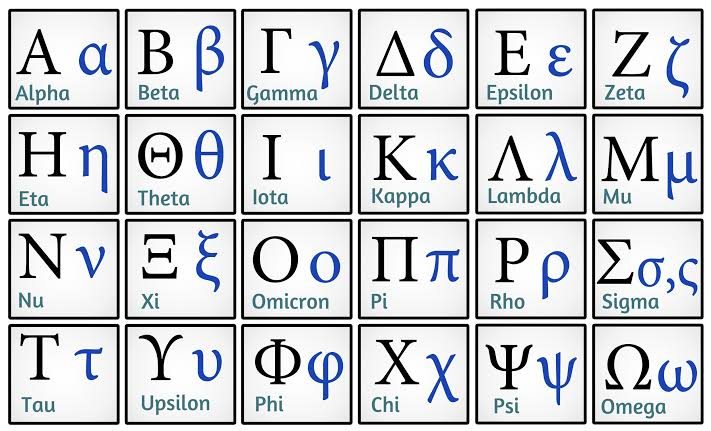
\includegraphics[width=5cm]{imagens/Alf_Grego.jpeg}
                \end{center}
            \end{figure}
        \end{enumerate}
    \end{frame}
    
    % Slide 3
    \begin{frame}{Analizando...}
        \begin{block}{$\varphi(x) = 2x + 1$}
            Variáveis: x
            \newline
            Constantes: 2; 1
            \begin{itemize}
                \item \textbf{Se x = 2:}
                \newline
                $2 * 2 + 1 = 5$
                \newline
                \item \textbf{Se x = 3:}
                \newline
                $2 * 3 + 1 = 7$
            \end{itemize}
        \end{block}
        \begin{alertblock}{Porque usar variáveis?}
            Se uso constantes provo somente para um caso, se uso variáveis provo para todos os casos, pois a variável está representando cada número do domínio a qual pertence.
        \end{alertblock}
    \end{frame}
    
    % Slide 4
    \begin{frame}
        \begin{center}
            
\includegraphics[width=5cm]{imagens/obrigado.jpg}
        \end{center}
        \begin{center}
            \textbf{Provérbios 1:7.a}
        \end{center}
        \begin{center}
            "O temor do Senhor é o princípio da ciência."
        \end{center}
    \end{frame}
    
\end{document}